\chapter{Implementación}

\section{Diseño del Sofware}

\noindent El diseño software no se ha orientado a crear un programa funcional para ser empleado por un usuario, sino que tiene como función entrenar los modelos probados y recabar los resultados oportunos de esos procesos. 

\medskip

\noindent En primer lugar se ha programado un \textit{notebook} de Jupyter independiente al proyecto general del framework, en el cual se realiza el preprocesamiento de los datos, la identificación de las caras y la separación en conjunto de entrenamiento y test. El fichero se denomina \textit{Make-crop-split database.ipynb}.

\medskip

\noindent Por otro lado, en lo que respecta al entrenamiento y diseño de la red, partíamos de un proyecto ya elaborado minuciosamente que se ha tenido que adaptar para aceptar como entrada la nueva base de datos así como alterar ciertas partes de su entrenamiento (para poder hacer el ajuste fino del decoder por ejemplo, realizar técnicas de \textit{cross validation 5-fold}) o introducir nuevos parámetros y funciones para la obtención y manipulación de los datos, y la generación de las gráficas y tablas de resultados que se muestran. Además se tuvieron que alterar las funciones del cálculo de métricas para que tuvieran en cuenta que en todas las imágenes no necesariamente se incluían todos los landmarks, y por lo tanto que solo computasen aquellos presentes en las mismas.

\begin{figure}[!h]
    \centering
    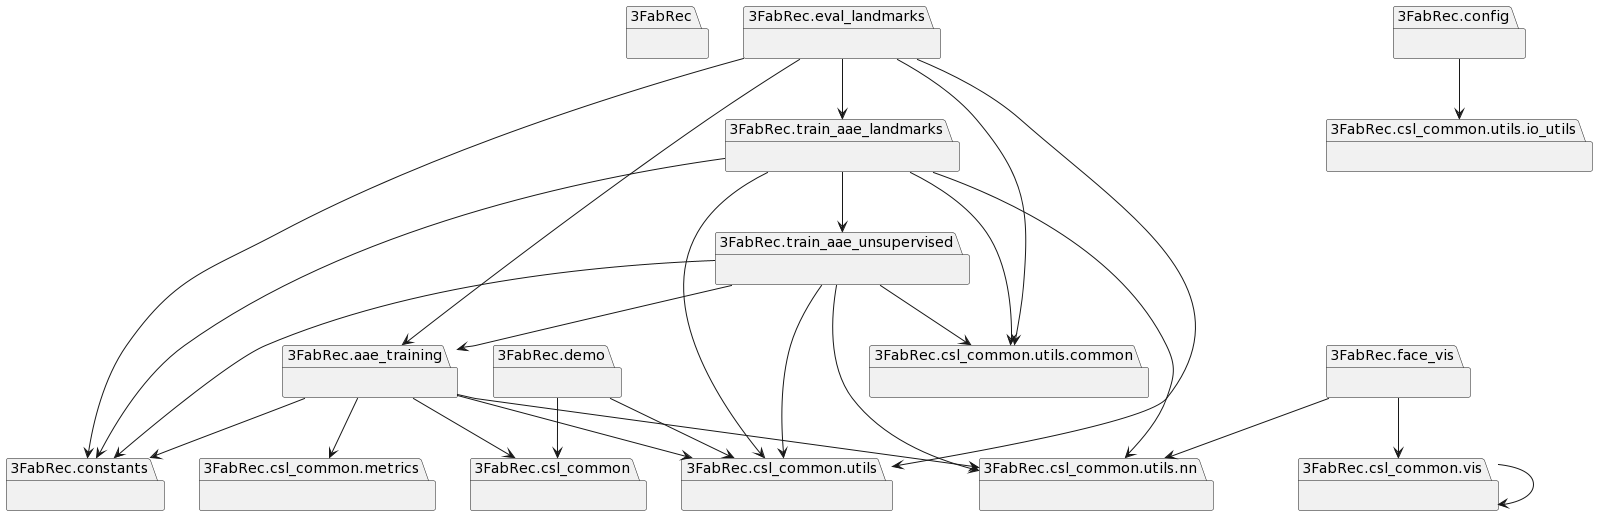
\includegraphics[width=0.9\textwidth]{img/diagrama_paquetes_1.png}
    \caption{Diagrama de paquetes del proyecto generado por \textit{pyreverse}, herramienta incluida en el paquete Pylint}
    \label{fig:Diagrama_paquetes}
\end{figure}

\medskip

\noindent En la imagen \autoref{fig:Diagrama_paquetes} podemos ver el diagrama de paquetes del proyecto. Dentro de dicho diagrama, el módulo que realiza el entrenamiento de la etapa supervisada (para la identificación de landmarks), se denomina \textit{train-aae-landmarks}. Y es configurado por una serie de parámetros que se introducen al programa desde la línea de comandos y que pueden consultarse los principales en la Tabla.

\begin{figure}[!h]
    \centering
    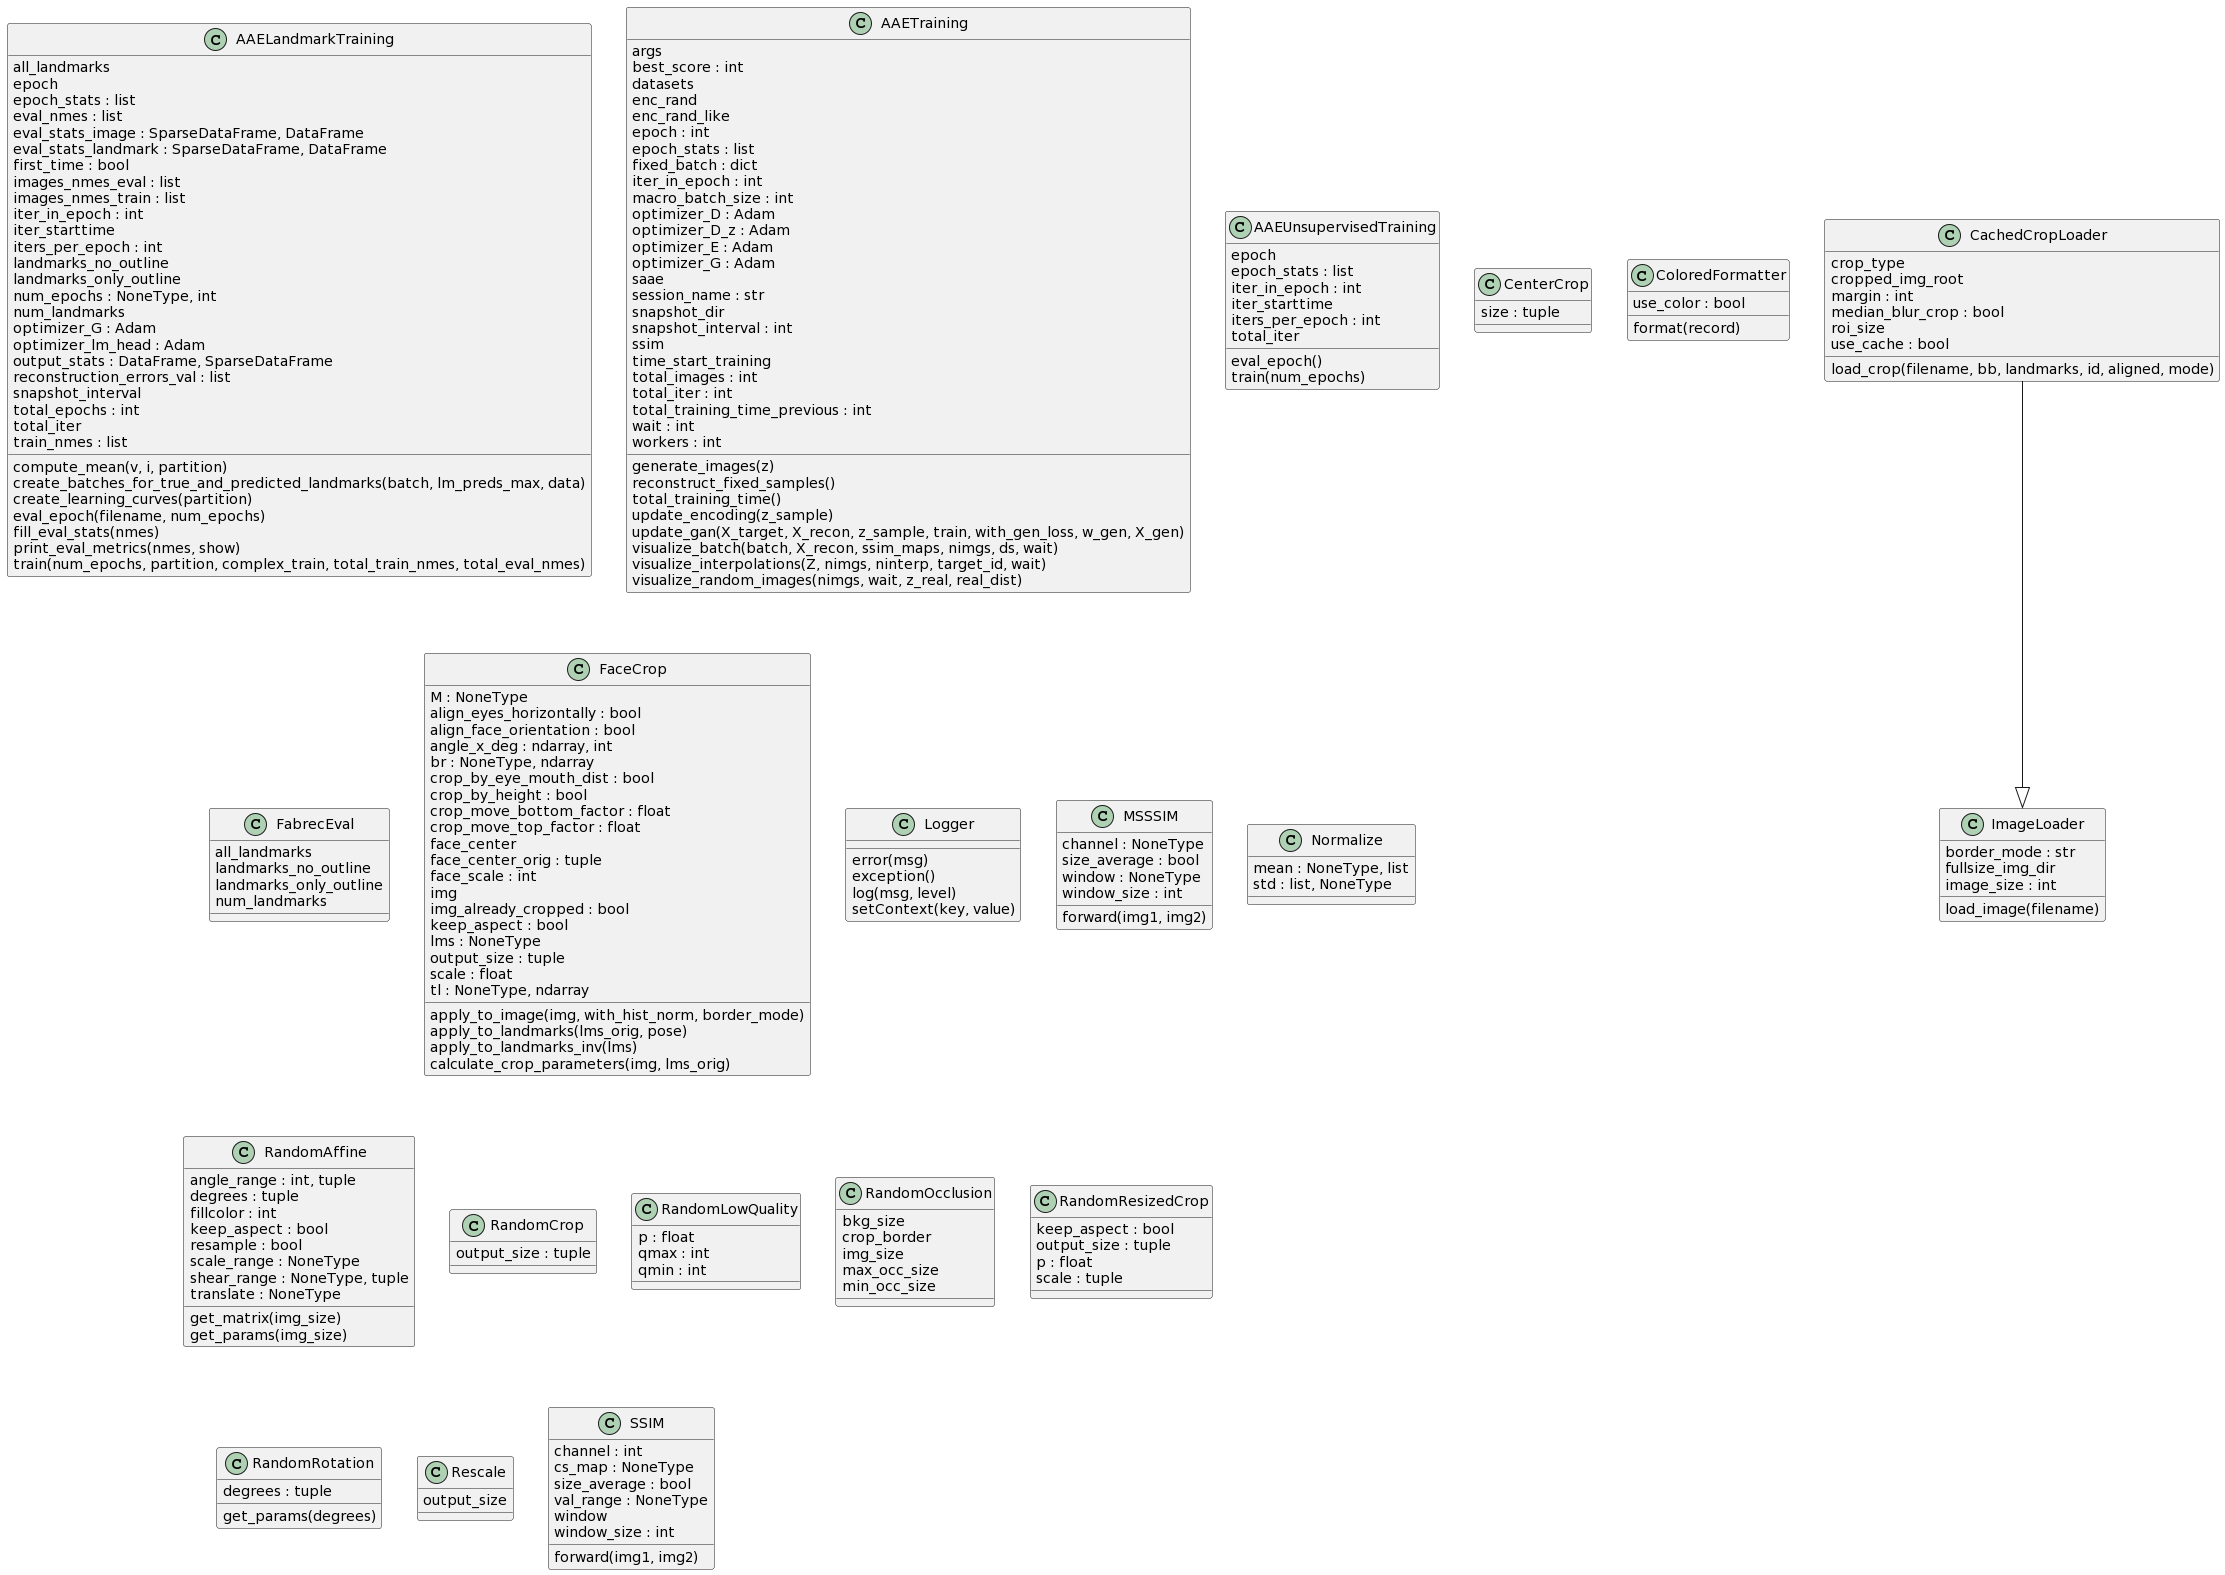
\includegraphics[width=0.9\textwidth]{img/diagrama_clases.png}
    \caption{Diagrama de clases con las principales clases del proyecto.}
    \label{fig:Diagrama_clases}
\end{figure}

\section{Entorno de ejecución}
\noindent Las ejecuciones se han realizado todas en un ordenador portátil \textit{HP Pavilion} con las siguientes características: 

\begin{itemize}
    \item Ubuntu $20.04.5$ LTS $64$ bits.
    \item $8$ GB de RAM
    \item $8$ x Intel® Core™ i$5$-$8300$H CPU @ $2.30$GHz
    \item GPU NVIDIA GeForce GTX $1050$ Mobile
\end{itemize}

\medskip

\noindent Por otro lado, las versiones del software empleado son: 

\begin{itemize}
    \item Python 3.6.13
    \item CUDA 10.1
    \item PyTorch 1.1.0
    \item Numpy 1.17.4
    \item Pandas 0.23.3
    \item Matplotlib 3.3.4
\end{itemize}


\endinput
%------------------------------------------------------------------------------------
% FIN DEL CAPÍTULO. 
%------------------------------------------------------------------------------------

